%%%%%%%%%%%%%%%%%%%%%%%%%%%%%%%%%%%%%%%%%
% Beamer Presentation
% LaTeX Template
% Version 1.0 (10/11/12)
%
% This template has been downloaded from:
% http://www.LaTeXTemplates.com
%
% License:
% CC BY-NC-SA 3.0 (http://creativecommons.org/licenses/by-nc-sa/3.0/)
%
%%%%%%%%%%%%%%%%%%%%%%%%%%%%%%%%%%%%%%%%%

%----------------------------------------------------------------------------------------
%	PACKAGES AND THEMES
%----------------------------------------------------------------------------------------

\documentclass{beamer}
\usepackage{fancyvrb}
\mode<presentation> {

% The Beamer class comes with a number of default slide themes
% which change the colors and layouts of slides. Below this is a list
% of all the themes, uncomment each in turn to see what they look like.

\usetheme{default}
%\usetheme{AnnArbor}
%\usetheme{Antibes}
%\usetheme{Bergen}
%\usetheme{Berkeley}
%\usetheme{Berlin}
%\usetheme{Boadilla}
%\usetheme{CambridgeUS}
%\usetheme{Copenhagen}
%\usetheme{Darmstadt}
%\usetheme{Dresden}
%\usetheme{Frankfurt}
%\usetheme{Goettingen}
%\usetheme{Hannover}
%\usetheme{Ilmenau}
%\usetheme{JuanLesPins}
%\usetheme{Luebeck}
%\usetheme{Madrid}
%\usetheme{Malmoe}
%\usetheme{Marburg}
%\usetheme{Montpellier}
%\usetheme{PaloAlto}
%\usetheme{Pittsburgh}
%\usetheme{Rochester}
%\usetheme{Singapore}
%\usetheme{Szeged}
%\usetheme{Warsaw}

% As well as themes, the Beamer class has a number of color themes
% for any slide theme. Uncomment each of these in turn to see how it
% changes the colors of your current slide theme.

%\usecolortheme{albatross}
%\usecolortheme{beaver}
%\usecolortheme{beetle}
\usecolortheme{crane}
%\usecolortheme{dolphin}
%\usecolortheme{dove}
%\usecolortheme{fly}
%\usecolortheme{lily}
%\usecolortheme{orchid}
%\usecolortheme{rose}
%\usecolortheme{seagull}
%\usecolortheme{seahorse}
%\usecolortheme{whale}
%\usecolortheme{wolverine}

%\setbeamertemplate{footline} % To remove the footer line in all slides uncomment this line
%\setbeamertemplate{footline}[page number] % To replace the footer line in all slides with a simple slide count uncomment this line

\setbeamertemplate{navigation symbols}{} % To remove the navigation symbols from the bottom of all slides uncomment this line
}

\usepackage{graphicx} % Allows including images
\usepackage{booktabs} % Allows the use of \toprule, \midrule and \bottomrule in tables

%----------------------------------------------------------------------------------------
%	TITLE PAGE
%----------------------------------------------------------------------------------------

\title[GDB]{Discussion Session 05} % The short title appears at the bottom of every slide, the full title is only on the title page

\author{Claudio Parra} % Your name
\institute[UCI] % Your institution as it will appear on the bottom of every slide, may be shorthand to save space
{
University of California \\ % Your institution for the title page
\medskip
\textit{parraca@uci.edu} % Your email address
}
\date{\today} % Date, can be changed to a custom date

\begin{document}

\begin{frame}
\titlepage % Print the title page as the first slide
\end{frame}

%\begin{frame}
%\frametitle{Overview} % Table of contents slide, comment this block out to remove it
%\tableofcontents % Throughout your presentation, if you choose to use \section{} and \subsection{} commands, these will automatically be printed on this slide as an overview of your presentation
%\end{frame}

%----------------------------------------------------------------------------------------
%	PRESENTATION SLIDES
%----------------------------------------------------------------------------------------

%------------------------------------------------
\section{First Section} % Sections can be created in order to organize your presentation into discrete blocks, all sections and subsections are automatically printed in the table of contents as an overview of the talk
%------------------------------------------------

\subsection{Subsection Example} % A subsection can be created just before a set of slides with a common theme to further break down your presentation into chunks

\begin{frame}
  \frametitle{Previously}
  QEMU
  \begin{itemize}
  \item Download (git clone)
  \item Configure
  \item Compile
  \item Install
  \item Modify \texttt{\$PATH}
  \end{itemize}
  Xv6
  \begin{itemize}
  \item Download (git clone)
  \item Compile
  \end{itemize}
\end{frame}

%------------------------------------------------

\begin{frame}
  \frametitle{make tool}
  \texttt{\centerline{make qemu-nox}}
  \begin{itemize}
  \item What are we doing? telling the tool \texttt{make} to read the \texttt{Makefile} script and run the target \texttt{quemu-nox}
  \item Possible error: qemu is not in the path.
  \end{itemize}
\end{frame}

%------------------------------------------------

\begin{frame}
%\frametitle{Big Picture}
\begin{figure}
  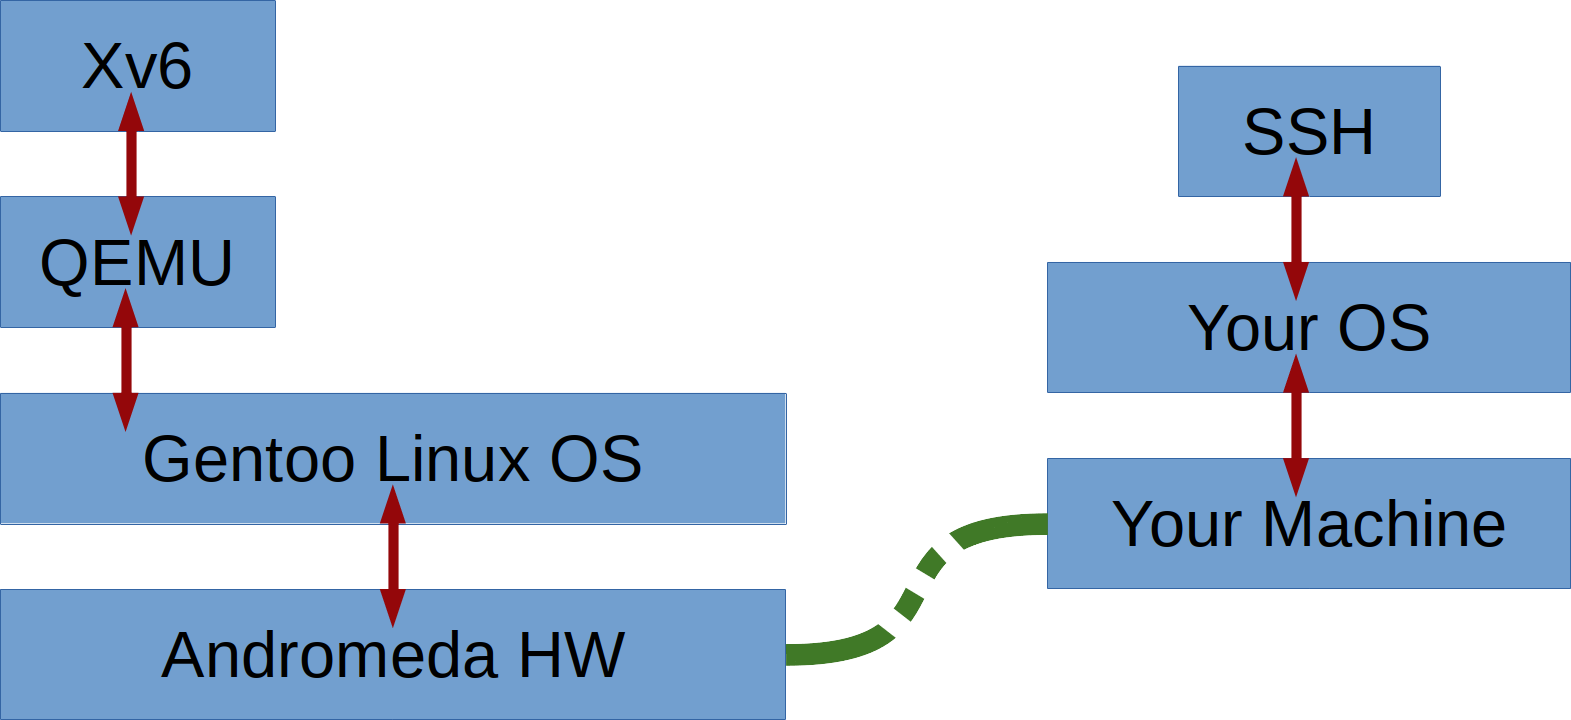
\includegraphics[width=0.8\linewidth]{bigpic-0}
  \caption{\texttt{make qemu-nox}}
\end{figure}
\end{frame}

%------------------------------------------------

\begin{frame}
  \frametitle{make tool}
  \texttt{\centerline{make qemu-nox-gdb}}
  \begin{itemize}
  \item What are we doing? telling the tool \texttt{make} to read the \texttt{Makefile} script and run the target \texttt{quemu-nox-gdb}
  \item Possible error: qemu is not in the path.
  \end{itemize}
\end{frame}

%------------------------------------------------

\begin{frame}
%\frametitle{Big Picture}
\begin{figure}
  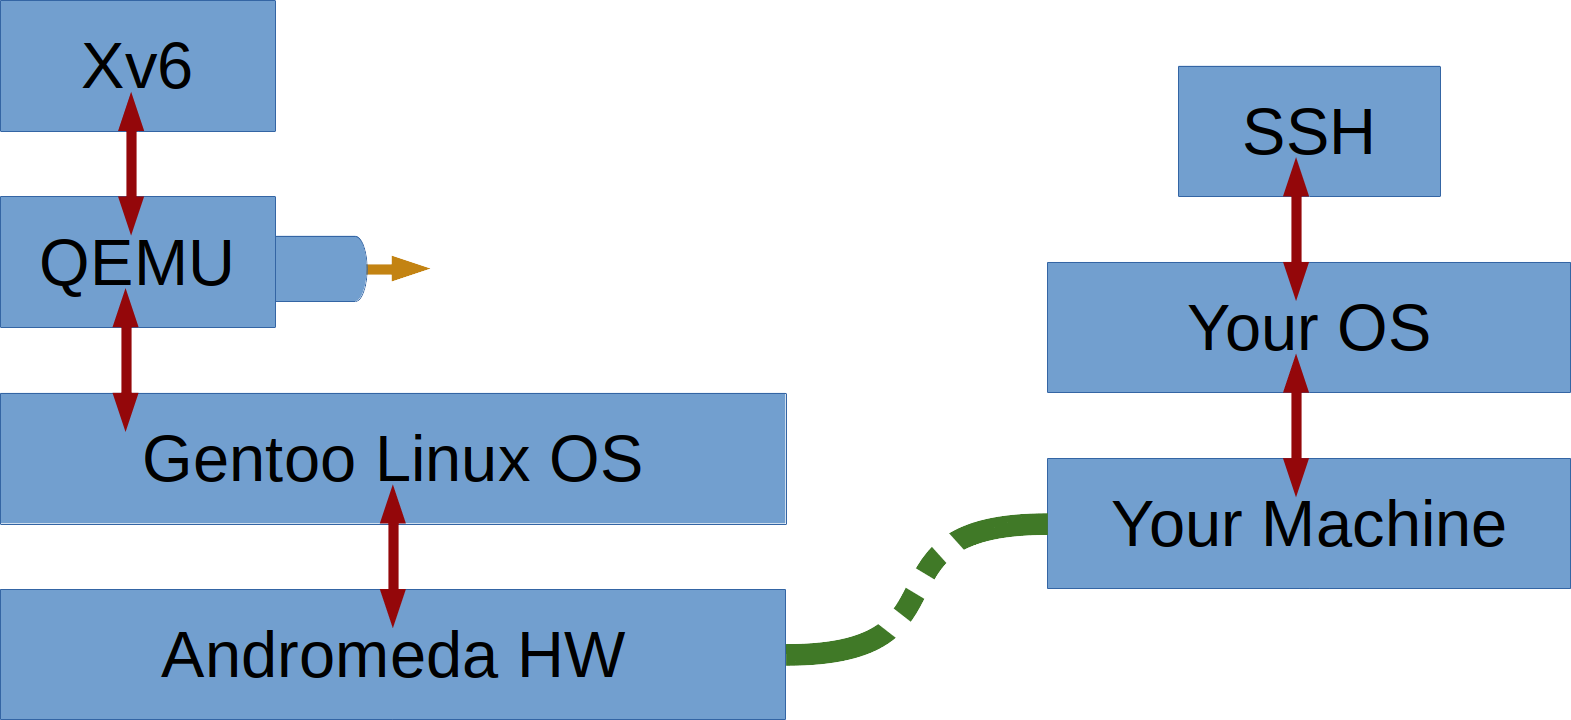
\includegraphics[width=0.8\linewidth]{bigpic-1}
  \caption{\texttt{make qemu-nox-gdb}}
\end{figure}
\end{frame}

%------------------------------------------------

\begin{frame}[fragile]
  \frametitle{gdb}
  \texttt{\centerline{gdb}}
  \begin{itemize}
  \item From the folder where you compiled Xv6, we simply run \texttt{gdb}. It should notice the connection that qemu has.
  \item Possible error:
\begin{Verbatim}[fontsize=\footnotesize]
  warning: File "/home/.../xv6/.gdbinit" auto-loading has
  been declined by your 'auto-load safe-path' set to
  "\$debugdir:\$datadir/auto-load".
  
  To enable execution of this file add
	add-auto-load-safe-path /home/.../xv6/.gdbinit
  line to your configuration file "/home/user/.gdbinit".
        
  To completely disable this security...
\end{Verbatim}
  \end{itemize}
\end{frame}

%------------------------------------------------

\begin{frame}
%\frametitle{Big Picture}
\begin{figure}
  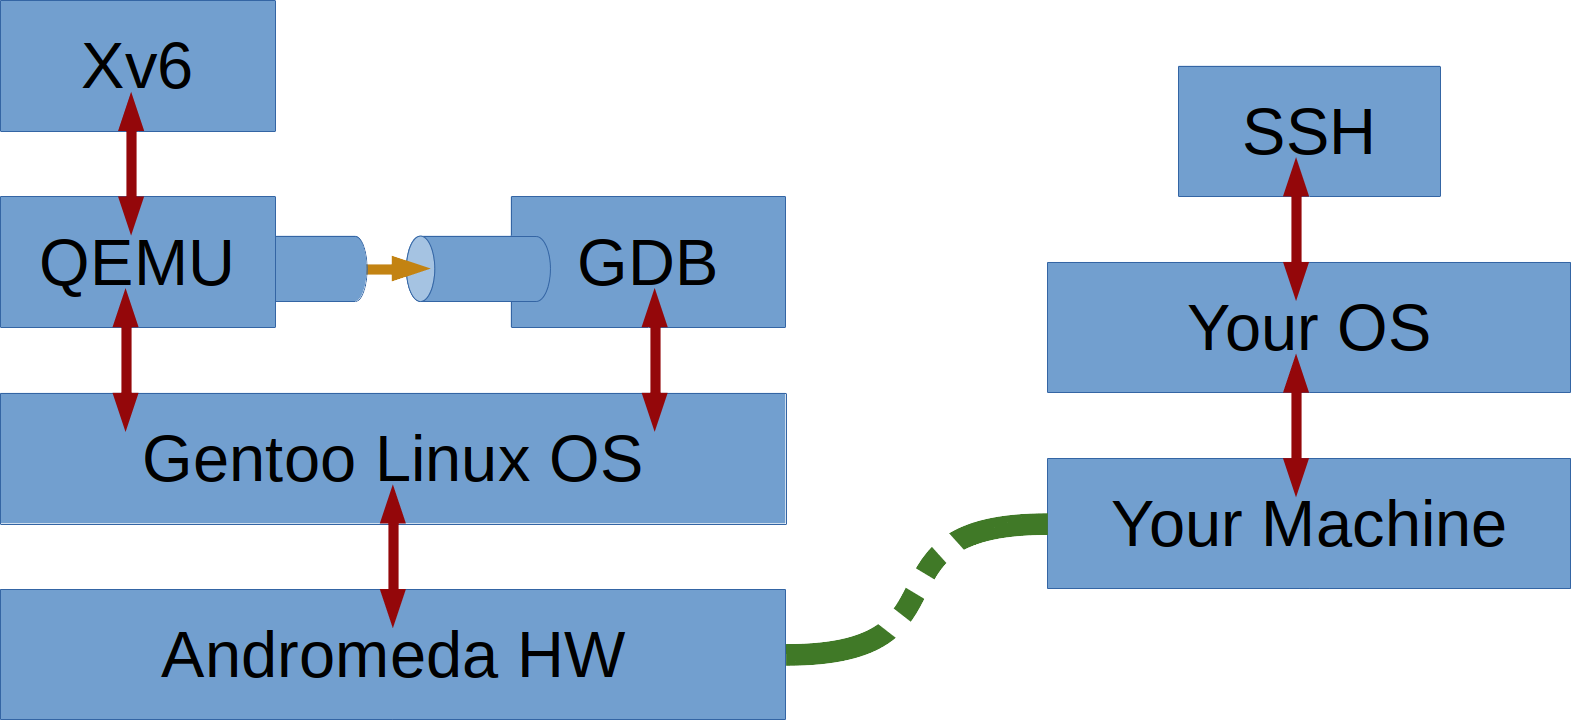
\includegraphics[width=0.8\linewidth]{bigpic-2}
  \caption{\texttt{gdb}}
\end{figure}
\end{frame}

%----------------------------------------------------------------------------------------

\end{document} 